\section{Mixed Practice}

\subsection{Warm Ups}
These are good problems for reinforcing the vocabulary and foundational concepts of this chapter.

\begin{exercise}{\Coffeecup }
\begin{enumerate}[label=\alph*.)]
\item Compare the growth orders of $x^2$ and $e^x$. 
\solushun{ $\lim\limits_{x \rightarrow \infty}{\frac{x^2}{e^{x}}} \stackrel{\text{H}}{=} \lim\limits_{x \rightarrow \infty}{ \frac{2x}{e^{x}}} \stackrel{\text{H}}{=} \lim\limits_{x \rightarrow \infty} {\frac{2}{e^{x}}}=0 \Longrightarrow e^{x}>>x^2 
$ 
\\ }{0in}
\item Compare the growth orders of $x^3$ and $e^x$.  
\solushun{ $\lim\limits_{x \rightarrow \infty}{\frac{x^3}{e^{x}}} \stackrel{\text{H}}{=} \lim\limits_{x \rightarrow \infty}{ \frac{3x^2}{e^{x}}} \stackrel{\text{H}}{=} \lim\limits_{x \rightarrow \infty} {\frac{6x}{e^{x}}}\stackrel{\text{H}}{=} \lim\limits_{x \rightarrow \infty} {\frac{6}{e^{x}}}=0 \Longrightarrow e^{x}>>x^3 
$ 
\\ }{0in}
\item Compare the growth orders of $x^4$ and $e^x$.  
\solushun{ $\lim\limits_{x \rightarrow \infty}{\frac{x^4}{e^{x}}} \stackrel{\text{H}}{=} \lim\limits_{x \rightarrow \infty}{ \frac{4x^3}{e^{x}}} \stackrel{\text{H}}{=} \lim\limits_{x \rightarrow \infty} {\frac{12x^2}{e^{x}}} \stackrel{\text{H}}{=} \lim\limits_{x \rightarrow \infty} {\frac{24x}{e^{x}}} \stackrel{\text{H}}{=} \lim\limits_{x \rightarrow \infty} {\frac{24}{e^{x}}}=0 \Longrightarrow e^{x}>>x^4
$ 
\\ }{0in}
\item Let $p(x)$ be a generic polynomial of degree $n$ where $n$ is a natural number.  What can you say about the growth order of $p(x)$ versus the growth order of $e^x$?  
\solushun{The above calculations demonstrate that if you compare $p(x)$ to $e^x$ you will have n iterations of LHR resulting in $\lim\limits_{x \to \infty}{\frac{p(x)}{e^x}}=\lim\limits_{x \to \infty}{\frac{n!}{e^x}}=0$ Thus $e^x$ has larger growth order than any polynomial.
\\ }{0in}
\end{enumerate}
\AnswerKeyEntry{a.~~ $e^{x}>>x^2$ 
b.~~ $e^{x}>>x^3$ 
c.~~$ e^{x}>>x^4$ 
d.~~The above calculations demonstrate that if you compare $p(x)$ to $e^x$ you will have n iterations of LHR resulting in $\lim\limits_{x \to \infty}{\frac{p(x)}{e^x}}=\lim\limits_{x \to \infty}{\frac{n!}{e^x}}=0$ Thus $e^x$ has larger growth order than any polynomial.
}
\end{exercise}

\begin{exercise}{\Coffeecup \Coffeecup }
Suppose a pyramid has height 3 and has an isosceles equilateral triangle with legs of length 2 for its base.  Find the volume $V$ of the pyramid using cross sections.
\AnswerKeyEntry{$V=9$}
\solushun{First we need to examine a cross-section of the pyramid.  Assume we set the pyramid so that the y-axis goes through the center of the base and the top vertex.  Then the base has area $A_{base} = \frac{1}{2}\cdot \sqrt{3} \cdot 2$ since the area of a triangle is $\frac{1}{2}bh$ and the altitude of an equilateral triangle with length of a side = s, is always $h=\frac{\sqrt{3}}{2} s$, then a general formula for area of an equilateral triangle is $\frac{1}{2}\frac{\sqrt{3}}{2} (s)^2$ \\
Note as we go up the pyramid, the length of a side of the equilateral triangle will decrease proportionally with the height.  So if we are at a generic point y, the length of a side $s(y)$ can be determined by $\frac{s(y)}{2} = \frac{3-y}{3}$  Thus $s(y) = \frac{2}{3}(3-y)$\\
We can use this to find the area of a any cross section at y on the pyramid to be:$A(y) = \frac{1}{2} \cdot \frac{\sqrt{3}}{2}[s(y)]^2 $ \\
Now we can integrate over y and get the volume:\\
$V= \int_0^3{ \frac{\sqrt{3}}{4}\left[\frac{2}{3}(3-y)\right]^2 dy}=\frac{\sqrt{3}}{9}\int_0^3{(9-6y+y^2) dy}=\frac{\sqrt{3}}{9} \left(9y-3y^2+\frac{y^3}{3}\right) \Biggr|_0^3=\frac{\sqrt{3}}{9}\left(27-27+9\right) -0 = 9$
\\ }{0in}
\end{exercise}

\begin{exercise}{\Coffeecup \Coffeecup }
Let $f(x) = \sqrt{4-(x-1)^2}$, and let $R$ be the region between the graph and the $x$-axis.  Find the volume $V$ of the solid obtained by revolving $R$ about the $y$-axis.
\AnswerKeyEntry{$V=\frac{\pi}{4} -\frac{\sqrt{2}}{6}$}
\solushun{Think of the solid as the top half of a torus.  The function gives us the bounds (or the width) of the region by solving for the x intercepts $\sqrt{4-(x-1)^2}=0 \Longrightarrow x= 0,3 $.  The height is $f(x) =\sqrt{4-(x-1)^2}$ \\
So we have $V = \int_0^3{2 \pi x \sqrt{4-(x-1)^2} dx} $\\
which we can solve with trig substitution. Let $x-1 = 2\sin{u}$ then $dx=2\cos{u} du$ we now have: \\
$\int_{-\pi/4}^{\pi/2}{2 \pi (2\sin{u}+1) \sqrt{4-4\sin^2{u}} 2\cos{u} ~du}= \int_{-\pi/4}^{\pi/2}{2 \pi (2\sin{u}+1) \sqrt{4\cos^2{u}} 2\cos{u} ~du}=4 \pi\int_{-\pi/4}^{\pi/2}{ (2\sin{u}+1) 2\cos^2{u} ~du}=8 \pi\int_{-\pi/4}^{\pi/2}{ (2\sin{u}\cos^2{u}+\cos^2{u})~du}=8 \pi \left[\int_{-\pi/4}^{\pi/2}{ 2\sin{u}\cos^2{u}~du} + \int_{-\pi/4}^{\pi/2}{\cos^2{u} ~du}  \right]=8 \pi \left[\int_{-\pi/4}^{\pi/2}{ 2\sin{u}\cos^2{u}~du} + \int_{-\pi/4}^{\pi/2}{\frac{1+\cos{2u}}{2} ~du}  \right]=8 \pi \left[ \frac{-2\cos^3{u}}{3} + \frac{1}{2} (u+\frac{\sin{2u}}{2})  \right] \Biggr|_{-\pi/4}^{\pi/2}$\\
$=8 \pi \left[ \left(\frac{-2\cos^3{\left(\pi/2\right)}}{3} + \frac{1}{2} (\frac{\pi}{2}+\frac{\sin{\left(\pi \right)}}{2})\right)-\left(\frac{-2\cos^3{\left(-\pi/4\right)}}{3} + \frac{1}{2} (\frac{-\pi}{4}+\frac{\sin{\left(\pi/2\right)}}{2})\right)  \right]$\\
$= 8\pi \left[ \left( 0 + \frac{\pi}{8} +\frac{1}{4} \right) - \left(\frac{\sqrt{2}}{6}-\frac{\pi}{8}+\frac{1}{4}\right) \right]=\frac{\pi}{4} -\frac{\sqrt{2}}{6}$
\\ }{0in}
\end{exercise}

\begin{exercise}{\Coffeecup \Coffeecup }
\begin{enumerate}[label=\alph*.)]
\item Sketch the region bounded by the following equations:
$$y=0$$
$$x=0$$
$$x=3$$
$$y = \frac{1}{(x+1)(x-3)^2}$$
\solushun{ 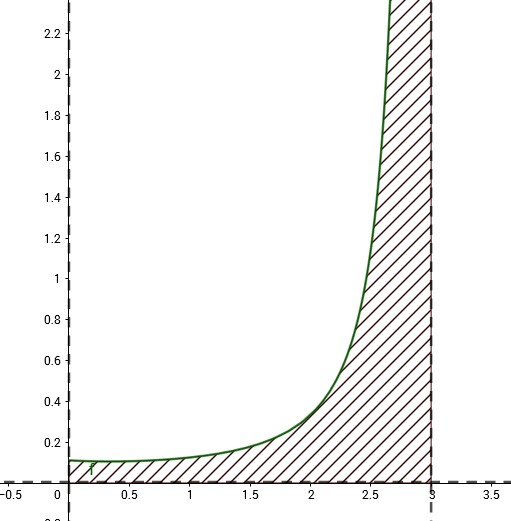
\includegraphics[scale=0.35]{ChapterGeom/Figures/mixedpracticepic1.jpg}
\\ }{0in}
\item Use an improper integral to find the area of the region.
\AnswerKeyEntry{The area is infinite!}
\solushun{ Note we will need PFD to integrate so first:\\
$\frac{1}{(x+1)(x-3)^2} = \frac{A}{(x-+1)}+\frac{B}{(x-3)}+\frac{C}{(x-3)^2} \Longrightarrow 1 = A(x-3)^2 + B(x+1)(x-3) +C(x+1)$ \\
Set $x=3$ then $1=C\cdot 4\Longrightarrow C=\frac{1}{4}$\\
Set $x=1$ then $1=A(-4)^2 \Longrightarrow A=\frac{1}{16}$\\
Use degree 2 coefficients then $A+B=0 \Longrightarrow B=-\frac{1}{16}$\\
$\int_0^3{\frac{1}{(x+1)(x-3)^2}dx}=\lim\limits_{c \rightarrow 3^{-}}{\int_0^c{\frac{1}{(x+1)(x-3)^2}dx}}=\lim\limits_{c \rightarrow 3^{-}}{\int_0^c{\frac{\frac{1}{16}}{(x+1)}+\frac{-\frac{1}{16}}{(x-3)}+\frac{\frac{1}{4}}{(x-3)^2}}dx}=\lim\limits_{c \rightarrow 3^{-}}{\frac{1}{16}}\ln{|x+1|}-\frac{1}{16}\ln{|x-3|}-\frac{1}{4}\frac{1}{(x-3)}\Biggr|_0^c$\\
$=\lim\limits_{c \rightarrow 3^{-}}{\left(\frac{1}{16}\ln{|c+1|}-\frac{1}{16}\ln{|c-3|}-\frac{1}{4}\frac{1}{(c-3)}\right)-\left(-\frac{1}{16}\ln{3}+\frac{1}{12}\right)}
$\\
As $c \rightarrow 3^{-}, ~~c-3 \rightarrow 0^{-}$. Thus $\ln{|c-3|} \rightarrow -\infty$, so $-\frac{1}{16}\ln{|c-3|} \rightarrow \infty $. Also, $-\frac{1}{4}\frac{1}{(c-3)} \rightarrow \infty$.  All the rest are constants.  Since we are adding 2 positive infinities and a big pile of constants we get $\infty$ Thus $A=\infty$
\\ }{0in}
\end{enumerate}

\end{exercise}

\begin{exercise}{\Coffeecup }
Demonstrate that the volume of a sphere is $V=\frac{4}{3}\pi r^3$ by cylindrical shells.
\AnswerKeyEntry{$V=\frac{4}{3} \pi r^3 $}
\solushun{The height of a shell is $2 f(x) = 2 \sqrt{r^2-x^2}$ and the radius is $x$. Thus the volume is $$V=\int_{x=0}														^{x=r}{2 \pi x \cdot 2 \sqrt{r^2-x^2} dx} ~~ $$Let $u=r^2-x^2$ Then $ du =-2x dx$ So 
$$ =4 \pi \int_{u=r^2}^{u=0}{x \sqrt{u} \frac{du}{-2x}}=2 \pi \int_{0}^{r^2}{u^{1/2}du} =2 \pi \frac{u^{3/2}}{3/2} \Biggr|_{0}^{r^2} = \frac{4}{3} \pi (r^2)^{3/2} = \frac{4}{3} \pi r^3 $$
\\ }{0in}
\end{exercise}

\begin{exercise}{\Coffeecup  }
Demonstrate that the volume of a sphere is $V=\frac{4}{3}\pi r^3$ by cross sections.
\AnswerKeyEntry{$V = \intop_{-r}^{r}{\pi (r^2-x^2) dx} =  \frac{4}{3} \pi r^3 $}
\solushun{Radius of a circular cross section is $f(x)$. Thus the area of the cross section is $\pi (f(x))^2 = \pi (r^2-x^2)$.  Now integrate: 
$$ V = \int_{x=-r}^{x=r}{\pi (r^2-x^2) dx} = (r^2x-x^3/3) \Biggr|_{-r}^{r} = \pi(r^3-r^3/3)-\pi(-r^3+r^3/3) = \pi(\frac{2}{3}r^3) + \pi(\frac{2}{3}r^3) = \frac{4}{3} \pi r^3
$$\\ }{0in}
\end{exercise}

\begin{exercise}{\Coffeecup \Coffeecup }
Calculate the center of mass of the region between the graphs of $f(x) =3x$ and $g(x) = x^2$ on the interval $[0,3]$. 
\AnswerKeyEntry{$\bar{x}=\frac{3}{2}, \bar{y}= \frac{18}{5} $}
\solushun{First note that the function $f(x) =3x $ is always greater than $g(x) =x^2$ on the interval given and the interval actually represents the intersection of the two functions.  Next calculate the area of the region.\\
$A= \int_0^3{3x-x^2~dx} = \frac{3x^2}{2} -\frac{x^3}{3} \Biggr|_0^3  = \left(\frac{27}{2} -\frac{27}{3} \right) -0 = \frac{9}{2}$\\
Now calculate $\bar{x} = \frac{2}{9}\int_0^3{x(3x-x^2)~dx} =\frac{2}{9}\int_0^3{(3x^2-x^3)~dx}=\frac{2}{9} \left( x^3-\frac{x^4}{4}\right) \Biggr|_0^3 = \frac{2}{9}\left(27 - \frac{81}{4}\right) = \frac{3}{2}  $ \\
$\bar{y} = \frac{2}{9}\int_0^3{\frac{1}{2}(3x-x^2)(3x+x^2)~dx} =\frac{1}{9}\int_0^3{(9x^2-x^4)~dx}=\frac{1}{9} \left( 3x^3-\frac{x^5}{5}\right) \Biggr|_0^3 = \frac{1}{9}\left(81 - \frac{243}{5}\right) = \frac{18}{5}  $ \\
\\ }{0in}
\end{exercise}



\subsection{Sample Test Problems}
\begin{exercise}{\Coffeecup \Coffeecup \Coffeecup}
 Consider the following function: $$ f(x)=\frac{\ln{x}}{\sqrt{x}}$$
\begin{enumerate}[label=\alph*.)]
\item What is $\lim \limits_{x\rightarrow \infty}f(x)$?
\solushun{$\lim \limits_{x\rightarrow \infty}{\frac{\ln{x}}{\sqrt{x}}}\stackrel{\text{H}}{=} \lim \limits_{x\rightarrow \infty}{\frac{\frac{1}{x}}{\frac{1}{2\sqrt{x}}} }=\lim \limits_{x\rightarrow \infty}\frac{2\sqrt{x}}{x}=\lim \limits_{x\rightarrow \infty}{\frac{2}{\sqrt{x}}}=0$ 
\\ }{0in}
\item What is $\lim\limits_{x\rightarrow 0^+}f(x)$?

\solushun{$\lim\limits_{x\rightarrow 0^+}{\frac{\ln{x}}{\sqrt{x}}}= \frac{-\infty}{o^{+}} = -\infty $
\\ }{0in}
\item Sketch the graph of $f$.  Include the information gathered in parts a) and b), as well as the point $(1,f(1))$.
\solushun{ 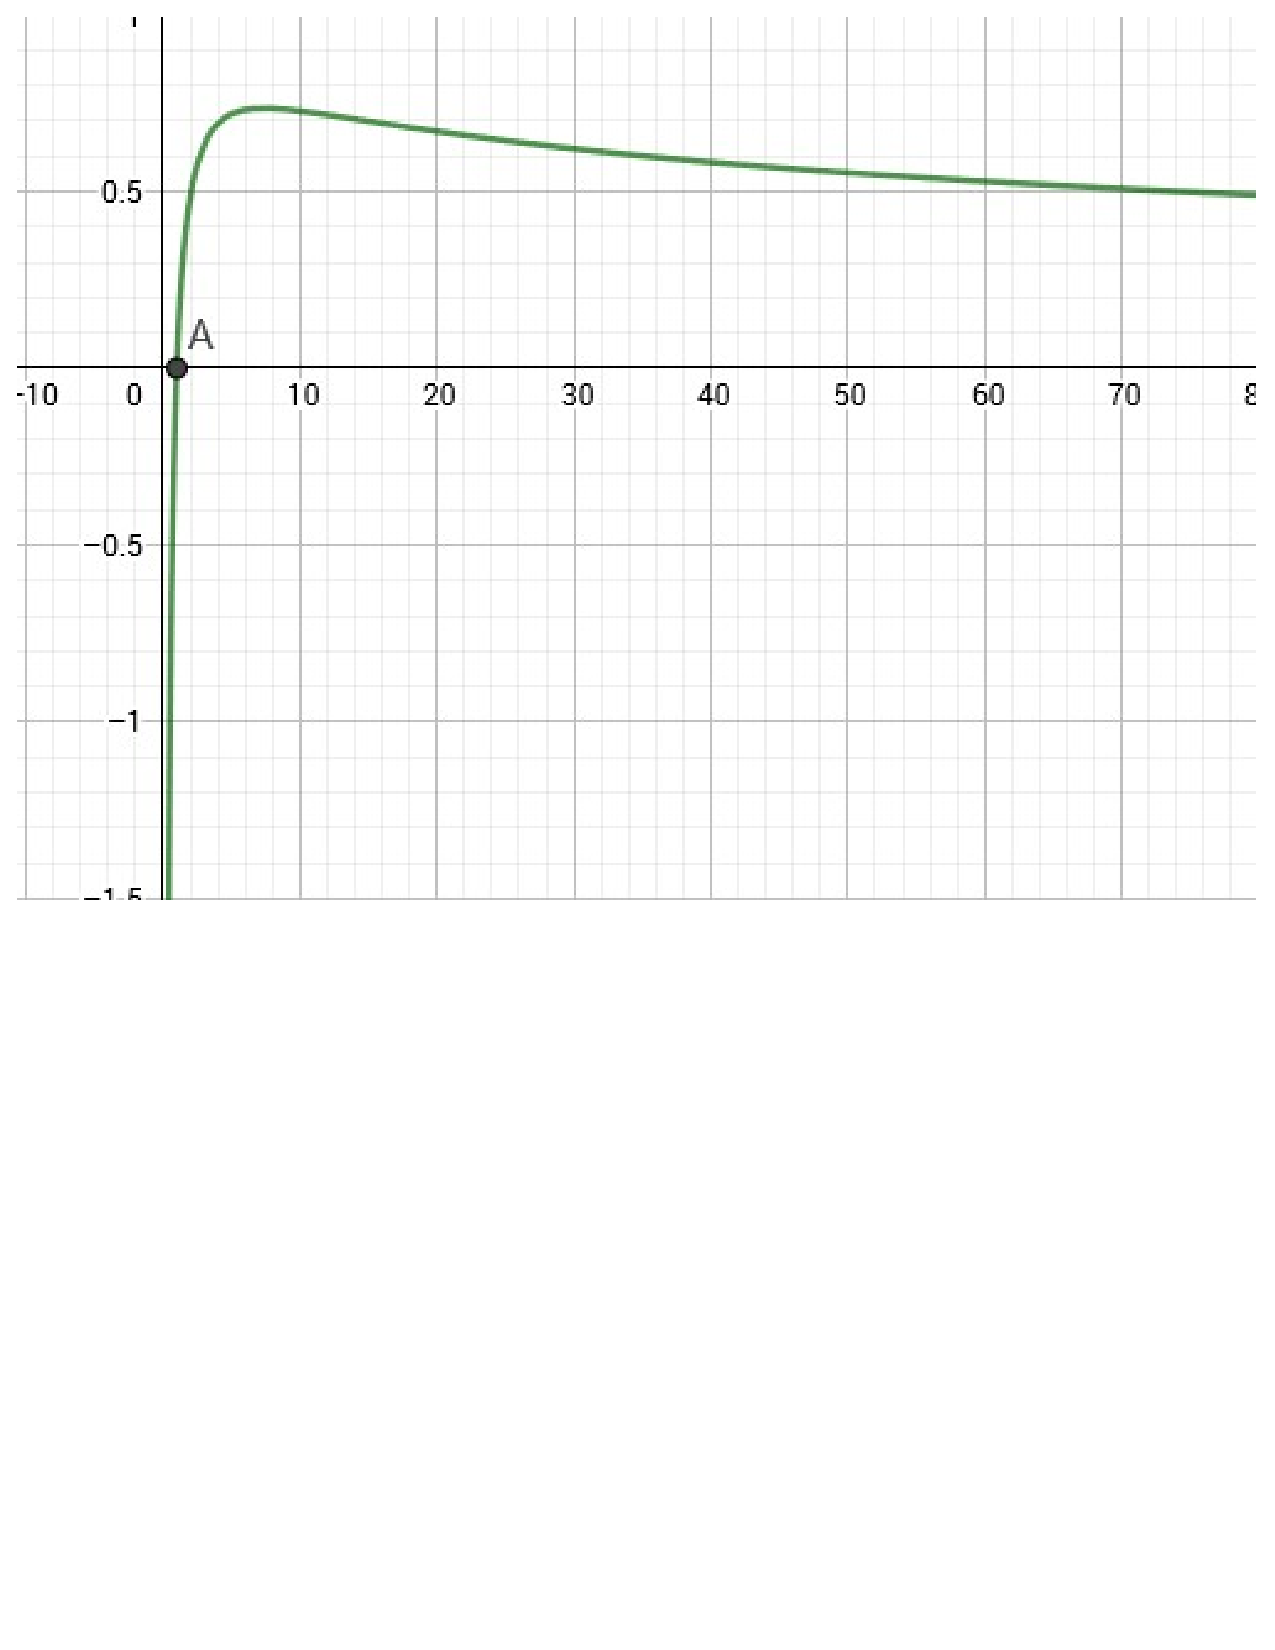
\includegraphics[scale=0.35]{ChapterGeom/Figures/lnoversqrt.pdf}
\\ }{0in}
\item Compute $\int_{0}^{1}{f(x)dx}$.  Interpret the result on your graph.
\AnswerKeyEntry{a.) $\lim \limits_{x\rightarrow \infty}{\frac{\ln{x}}{\sqrt{x}}}=0$ \newline
b.) $\lim \limits_{x\rightarrow 0^+}{\frac{\ln{x}}{\sqrt{x}}}=-\infty$\newline
d.) $\intop_{0}^{1}{\frac{\ln{x}}{\sqrt{x}}dx}=-4$
}
\solushun{ $\int_{0}^{1}{f(x)dx}=\int_{0}^{1}{\frac{\ln{x}}{\sqrt{x}}dx}$ \\
Use Integration by Parts with $u=\ln{x} \Rightarrow du=\frac{1}{x} dx$ \\
and $dv=x^{-1/2} dx \Rightarrow v = 2x^{1/2}$ \\
Let's start with the corresponding indefinite integral $\int{\frac{\ln{x}}{\sqrt{x}}dx} = 2x^{1/2} \ln{x}-2\int{x^{1/2}\frac{1}{x} dx}= 2x^{1/2} \ln{x}-2\int{x^{-1/2} dx}=2x^{1/2} \ln{x}-2(2)x^{1/2} +C=2x^{1/2}\ln{x}-4x^{1/2}+C$ \\ 
Now we address the bounds: $\int_0^1{\frac{\ln{x}}{\sqrt{x}}dx}= \lim \limits_{b \rightarrow 0^{+}}{\int_b^1 {\frac{\ln{x}}{\sqrt{x}}dx}}=\lim \limits_{b \rightarrow 0^{+}}{2x^{1/2}\ln{x}-4x^{1/2}} \Biggr|_b^1$ \\
$=-4 - \lim \limits_{b \rightarrow 0^{+}}{2b^{1/2}\ln{b}-0}$ \\
Note that we need L'Hospital's rule $\lim \limits_{b \rightarrow 0^{+}}{b^{1/2}\ln{b}}=\lim \limits_{b \rightarrow 0^{+}}{\frac{\ln{b}}{\frac{1}{b^{1/2}}}}=\lim \limits_{b \rightarrow 0^{+}}{\frac{\ln{b}}{b^{-1/2}}}\stackrel{\text{H}}{=}\lim \limits_{b \rightarrow 0^{+}}{\frac{\frac{1}{b}}{-\frac{1}{2} b^{-3/2}}}=\lim \limits_{b \rightarrow 0^{+}}{\frac{2b^{3/2}}{b}} =\lim \limits_{b \rightarrow 0^{+}}{2b^{1/2}} = 0$\\
So we get $\int_{0}^{1}{\frac{\ln{x}}{\sqrt{x}}dx}=-4$\\
The area is 4 but negative because it is under the x axis.
\\ }{0in}
\end{enumerate}
\end{exercise}


\begin{exercise}{\Coffeecup \Coffeecup \Coffeecup \Coffeecup}
\begin{enumerate}
\item Differentiate the function $$f(x)=\frac{1}{2}(x-1)\sqrt{x^2-2x}-\ln\left(\sqrt{x-2}+\sqrt{x}\right)$$ and verify that $$f'(x)=\sqrt{x^2-2x}.$$
\solushun{$f'(x) = \frac{1}{2} \left[ 1(x^2-2x)^{1/2} + \frac{1}{2}(x^2-2x)^{1/2}(2x-2)(x-1) \right] - \frac{\frac{1}{2(x-2)^{1/2}} +\frac{1}{2x^{1/2}}}{(x-2)^{1/2}+x^{1/2}} $ 
rewrite the first part and multiply the second part by $(2(x-2)^{1/2}x^{1/2} $ the common denominator and you get \\
$= \frac{1}{2}\left[(x-2x)^{1/2} + \frac{(x-1)^2}{(x^2-2x)^{1/2}} \right] - \frac{x^{1/2}+(x-2)^{1/2}}{2(x-2)x^{1/2}+2(x-2)^{1/2}x}$ \\
combine the fractions on the first part and factor the denominator on the second part \\
$\frac{1}{2} \left[\frac{x^2-2x+x^2-2x+1}{(x^2-2x)^{1/2}}\right]-\frac{x^{1/2}+(x-2)^{1/2}}{2x^{1/2}(x-2)^{1/2}((x-2)^{1/2}+x^{1/2})} $ \\
Now we can simplify the left part and cancel the numerator in the second part to get \\
$\frac{1}{2} \left[\frac{2x^2-4x+1}{(x^2-2x)^{1/2}}\right]-\frac{1}{2x^{1/2}(x-2)^{1/2}} $\\
notice the denominator of the first part $2(x^2-2x)^{1/2}$ is equal to the denominator of the second part $2x^{1/2}(x-2)^{1/2} = 2(x(x-2))^{1/2} = 2(x^2-2x)^{1/2}$\\
 combine these two  fractions and you get $ \frac{2x^2-4x}{2(x^2-2x)^{1/2}} = \frac{(x^2-2x)}{(x^2-2x)^{1/2}} = \sqrt{x^2-2x}$
\\ }{0in}
\item Find the length of $f(x)$ from $x=2$ to $x=4$.
\AnswerKeyEntry{ $4$}
\solushun{ Now that we have $f'(x)$ we can find the length using \\
$L=\int_2^4{\sqrt{1+[f'(x)]^2}dx}=\int_2^4{\sqrt{1+[\sqrt{x^2-2x}]^2}dx}=\int_2^4{\sqrt{1+x^2-2x}dx}=\int_2^4{\sqrt{(x-1)^2}dx}=\int_2^4{(x-1)dx}=\frac{x^2}{2}-x \Biggr|_2^4 =(8-4)-(2-2)=4$ \\ }{0in}
\end{enumerate}
\end{exercise}

\begin{exercise}{\Coffeecup \Coffeecup \Coffeecup}
\begin{enumerate}
\item Explain in words the difference between finding volume integrating via cylindrical shells vs via cross sections. 
\solushun{Cylindrical shells takes line segments and revolves them about an axis parallel to those segments in order to find the volume of the solid created by that revolution.  Cross sections cuts a 3D object into 2D parallel slices and does not require revolution. \\ }{0in}
\item Consider the tetrahedron with vertices at (0,0,0), (1,0,0), (0,1,0), and (0,0,1).
To find its volume, which of the above two methods would you use, and why?
\solushun{You cannot use shells because it is impossible to obtain a tetrahedron via revolution since it has no rotational symmetry.  So we use cross sections. \\ }{0in}
\item Find its volume using an integral.  
\AnswerKeyEntry{1. Cylindrical shells takes line segments and revolves them about an axis parallel to those segments in order to find the volume of the solid created by that revolution.  Cross sections cuts a 3D object into 2D parallel slices and does not require revolution.\newline
2. You cannot use shells because it is impossible to obtain a tetrahedron via revolution since it has no rotational symmetry.  So we use cross sections.\newline
3. $\intop_0^2 {\frac{1}{2}(1-2x+x^2)dx}=\frac{1}{6} $
}
\solushun{ At $x=0$ we have a $1 x 1$ right triangle, so the area is $\frac{1}{2}$. \\
At $x=1$, we have a $0 x 0$ point so the area is 0. \\
At any x-coordinate, the right triangle cross section has base $(1-x)$ and height $(1-x)$. Thus the area is $A(x) = \frac{1}{2}(1-x)(1-x) = \frac{1}{2}(1-2x+x^2)$.\\
We integrate to find volume:\\
$V= \int_0^2 {\frac{1}{2}(1-2x+x^2)dx}= \frac{1}{2} \int_0^1{ 1-2x+x^2 dx} = \frac{1}{2}(x-x^2 + \frac{x^3}{3} \Biggr|_0^1 = \frac{1}{2}(1-1+\frac{1}{3})-0 = \frac{1}{6} $\\ }{0in}
\end{enumerate}
\end{exercise}

\begin{exercise}{\Coffeecup \Coffeecup \Coffeecup }
\begin{enumerate}[label=\alph*.)]
\item Use integrals to find the center of mass of the first quadrant region bounded by $y=x$ and $y=x^n$, where $n \geq 1$.   Call this point $(\overline{x}_n,\overline{y}_n)$.
\solushun{First note that the function $f(x) =x$ is always greater than or equal to $g(x) = x^n$.  Also the intersection of the functions is at $x = 0$ and $x = 1$ First we find the area of the region $m = \int_0^1{x-x^n ~dx} = \frac{x^2}{2} - \frac{x^{n+1}}{n+1} \Biggr|_0^1 = \frac{1}{2} - \frac{1}{n+1} = \frac{n-1}{2(n+1)}$\\
Now we can calculate $\bar{x} = \frac{1}{m} \int_0^1{x(x-x^n)~dx} = \frac{2(n+1)}{n-1}\int_0^1{(x^2-x^{n+1})~dx}=\frac{2(n+1)}{n-1}\left( \frac{x^3}{3} - \frac{x^{n+2}}{n+2} \Biggr|_0^1 \right)=\frac{2(n+1)}{n-1}\left( \frac{1}{3} - \frac{1}{n+2} \right)=
\frac{2(n+1)}{n-1}  \frac{n-1}{3(n+2)} =\frac{2(n+1)}{3(n+2)}$\\
Also, we can calculate $\bar{y} = \frac{1}{m} \int_0^1{\frac{1}{2}(x-x^n)(x+x^n)~dx} = \frac{2(n+1)}{n-1}\int_0^1{\frac{1}{2}(x^2-x^{2n})~dx}=\frac{(n+1)}{n-1}\left( \frac{x^3}{3} - \frac{x^{2n+1}}{2n+1} \Biggr|_0^1 \right)=\frac{(n+1)}{n-1}\left( \frac{1}{3} - \frac{1}{2n+1} \right)=
\frac{(n+1)}{n-1}  \frac{2n-2}{3(2n+1)} =\frac{2(n+1)}{3(2n+1)}$\\
Thus the center of mass is $\left(\frac{2(n+1)}{3(n+2)},\frac{2(n+1)}{3(2n+1)}\right)$
\\ }{0in}
\item As $n\rightarrow \infty$, what point does $(\overline{x}_n,\overline{y}_n)$ approach?
\solushun{$\lim\limits_{x \to \infty}{\frac{2(n+1)}{3(n+2)}} = \frac{2}{3}$ and $\lim\limits_{x \to \infty}{=\frac{2(n+1)}{3(2n+1)}} = \frac{1}{3}$
\\ }{0in}
\item Use integrals to find the center of mass the triangle whose vertices are (0,0), (1,0), and (1,1).  How does this relate to your answer above?
\end{enumerate}
\AnswerKeyEntry{$\left(\frac{2}{3},\frac{1}{3} \right) $}
\solushun{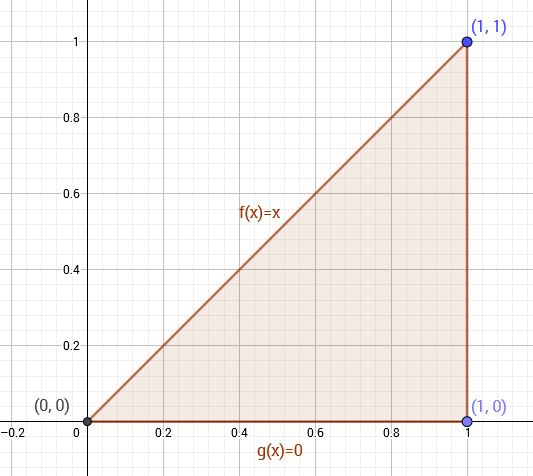
\includegraphics[scale=0.35]{ChapterGeom/Figures/mixedpracticepic2.jpg}\\
We calculate the area of the triangle $m = \frac{1}{2}\cdot 1 \cdot 1 = \frac{1}{2}$\\
Now calculate $\bar{x}$ and $\bar{y}$ using $f(x) = x$ and $g(x) = 0$.\\
$\bar{x} = 2 \int_0^1{x(x-0) ~dx} = \frac{2x^2}{3} \Biggr|_0^1 = \frac{2}{3}$ \\
$\bar{y} = 2 \int_0^1{\frac{1}{2}(x-0)(x+0)~dx}=\int_0^1{x^2~dx} = \frac{x^3}{3} \Biggr|_0^1=\frac{1}{3}$\\
So the center of mass is $\left(\frac{2}{3},\frac{1}{3} \right) $\\
This is related to the answer above because the function $x^n$ will approach the right angle side of the triangle as $n \rightarrow \infty$. So the center of mass will approach the center of mass of the triangle.\\ }{0in}
\end{exercise}


